\begin{circuitikz}[background rectangle/.style={fill=white}, show background rectangle]
        \node(0,0) {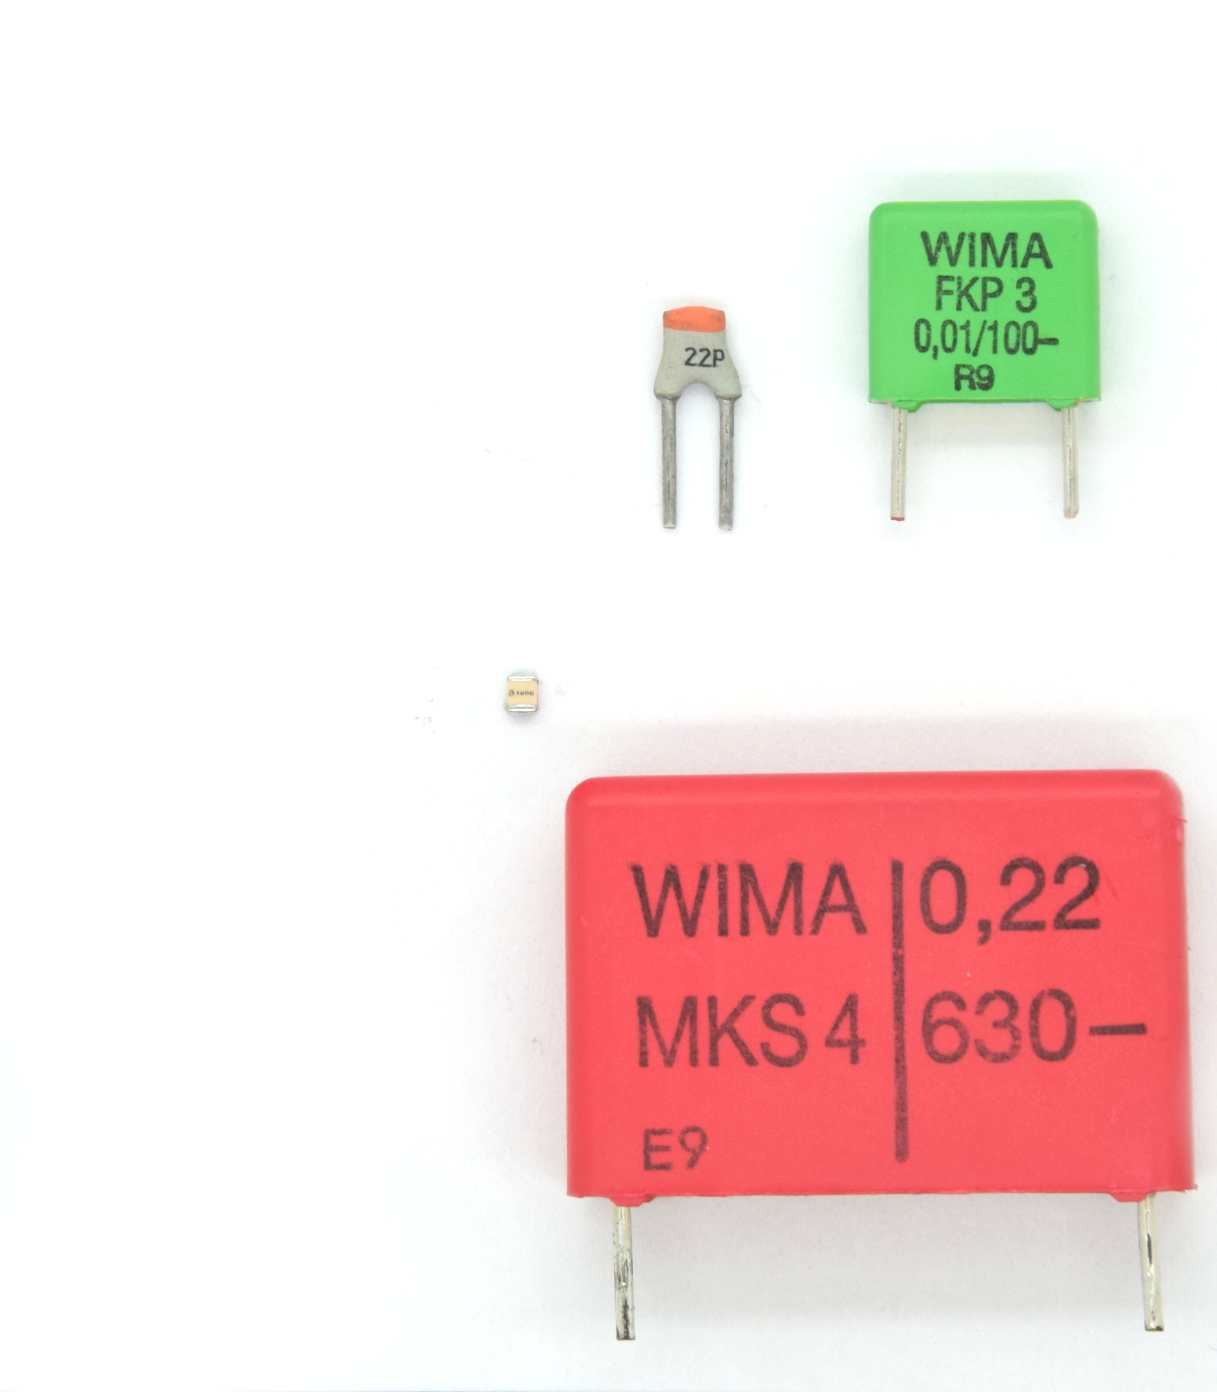
\includegraphics[width=200pt]{foto/8}};
        
        \draw(-3.0,1) to [C, european,l={$C$}] ++(0,-2);
    
        % Beschriftung:
        \draw( 2.20,  3.25) node {\small \qty{10}{\nano\farad}};
        \draw( 2.20,  0.75) node {\small \qty{100}{\volt}};
        \draw( 0.55,  2.50) node {\small \qty{22}{\pico\farad}};
        \draw( 0.55,  0.65) node {\small \qty{50}{\volt}};
        \draw( 1.55, -0.00) node {\small \qty{220}{\nano\farad}};
        \draw( 1.55, -3.50) node {\small \qty{630}{\volt}};
        \draw(-0.45,  0.25) node[right, rotate=90] {\small 0805 \qty{18}{\pico\farad} / \qty{50}{\volt}};
    
        % Pfeile:
        \draw[>=triangle 60, <->] (-1.6,0.675) coordinate(c1) -- ++(0,-1.35) coordinate(c2);
        \draw(c1) -- ++( 0.25,0);
        \draw(c1) -- ++(-0.25,0);
        \draw(c2) -- ++( 0.25,0);
        \draw(c2) -- ++(-0.25,0);
    
        % Text:
        \draw (c1) ++ (0,0.25) node {\qty{1}{\centi\meter}};
    
\end{circuitikz}